\documentclass[12pt,letterpaper]{article}
\usepackage[utf8]{inputenc}	% Para caracteres en español
\usepackage{amsmath,amsthm,amsfonts,amssymb,amscd}
\usepackage[table]{xcolor} 
\usepackage[margin=3cm]{geometry}
\usepackage{ragged2e}
\usepackage{graphicx}
\usepackage{hyperref}
\newlength{\tabcont}
\setlength{\parindent}{0.0in}
\setlength{\parskip}{0.05in}


\title{EP1}

\begin{document}
	
\begin{center}
	\large \bf
	Relatório do Exercício-Programa I de MAC0239 \\
\end{center}
	
\begin{table}[]
	\centering
	\label{my-label}
	\begin{tabular}{llll}
		\textbf{Nomes:} & Bruno Rafael Aricó        &\textbf{Nº USP:} & 8125459 \\
		& Isabela Blücher                 &         & 9298170 \\
		& Luís Felipe de Melo Costa Silva &         & 9297961 \\
		& Nícolas Nogueira Lopes da Silva &         & 9277541 \\
	\end{tabular}
\end{table}

\section{Problema}

\quad Tivemos que implementar um sistema de provas para o cálculo proposicional usando os tableaux semânticos (com as expansões $\alpha$ e $\beta$) para provar validade ou não de um sequente, da seguinte forma: 
\begin{center}
	$A_1, A_2, ..., A_n \vdash B$, onde:
\end{center}
As fórmulas $A_i, i = 1, 2, ..., n$ são as premissas e $B$ é a consequência. No caso de a fórmula ser inválida, devemos mostrar um contraexemplo.

\section{Implementação}

\quad O principal problema encontrado foi a análise léxica da entrada. Uma linguagem para as fórmulas foi definida no enunciado. Os parênteses são usados em todas as fórmulas e os átomos são do tipo $p, q$, etc. Os operadores foram definidos como:
	
\begin{itemize}
	\item .I. = $\to$ 
	\item .A. = $\land$
	\item .O. = $\lor$
	\item .N. = $\lnot$
\end{itemize}

\quad No entanto, não sabíamos como fazer um programa que entendesse essa linguagem. Para nos ajudar, usamos um analisador análogo ao FLEX para o C, o ANTLR.

\subsection{ANTLR}

\quad O \href{http://www.antlr.org/}{ANTLR} (ANother Tool for Language Recognition)
é um gerador de códigos para leitura, processamento, execução ou tradução de textos estruturados ou arquivos binários. É bastante usado para construir linguagens, ferramentas e arcabouços. A partir de uma gramática, ele gera um \textit{parser} que consegue construir e percorrer \textit{parse trees}.

\quad Usamos o ANTLR como base principal do nosso trabalho. A partir dos pedidos da ferramenta, criamos nossa gramática, definida no arquivo Expr.g4. Ele gera os arquivos necessários para o reconhrecimento da linguagem. Os arquivos gerados tem a forma Expr*.java.

\quad O arquivo EvalVisitor foi criado por nós e nele estão definidas as regras de expansão do Tableau. Atacamos o problema da seguinte forma:

DETALHES

\quad Uma curiosidade é que o ANTLR consegue gerar imagens a partir da linguagem e da entrada. Segue exemplo:

\begin{figure}[!h]
	\centering
	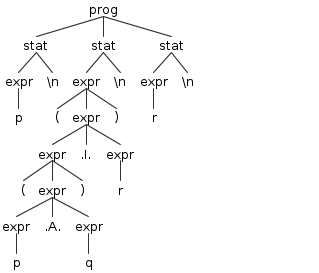
\includegraphics[scale=0.9]{1.png}
	\caption{Gerada com o comando \texttt{\$ java org.antlr.v4.gui.TestRig Expr prog -gui input}, onde \texttt{input} é o arquivo com a entrada}
\end{figure}

\quad 
\end{document}